\documentclass{article}

\usepackage{graphicx}
\usepackage{tikz}
\usepackage{tikzsymbols}
\usetikzlibrary{calc,patterns,shapes.geometric}
\pagestyle{empty}
\usepackage[margin=0pt]{geometry}
\geometry{papersize={14in,12in}}

\def\centerarc[#1](#2)(#3:#4:#5){\draw[#1] ($(#2)+({#5*cos(#3)},{#5*sin(#3)})$) arc (#3:#4:#5);}

\begin{document}
	\begin{figure}
		\centering
		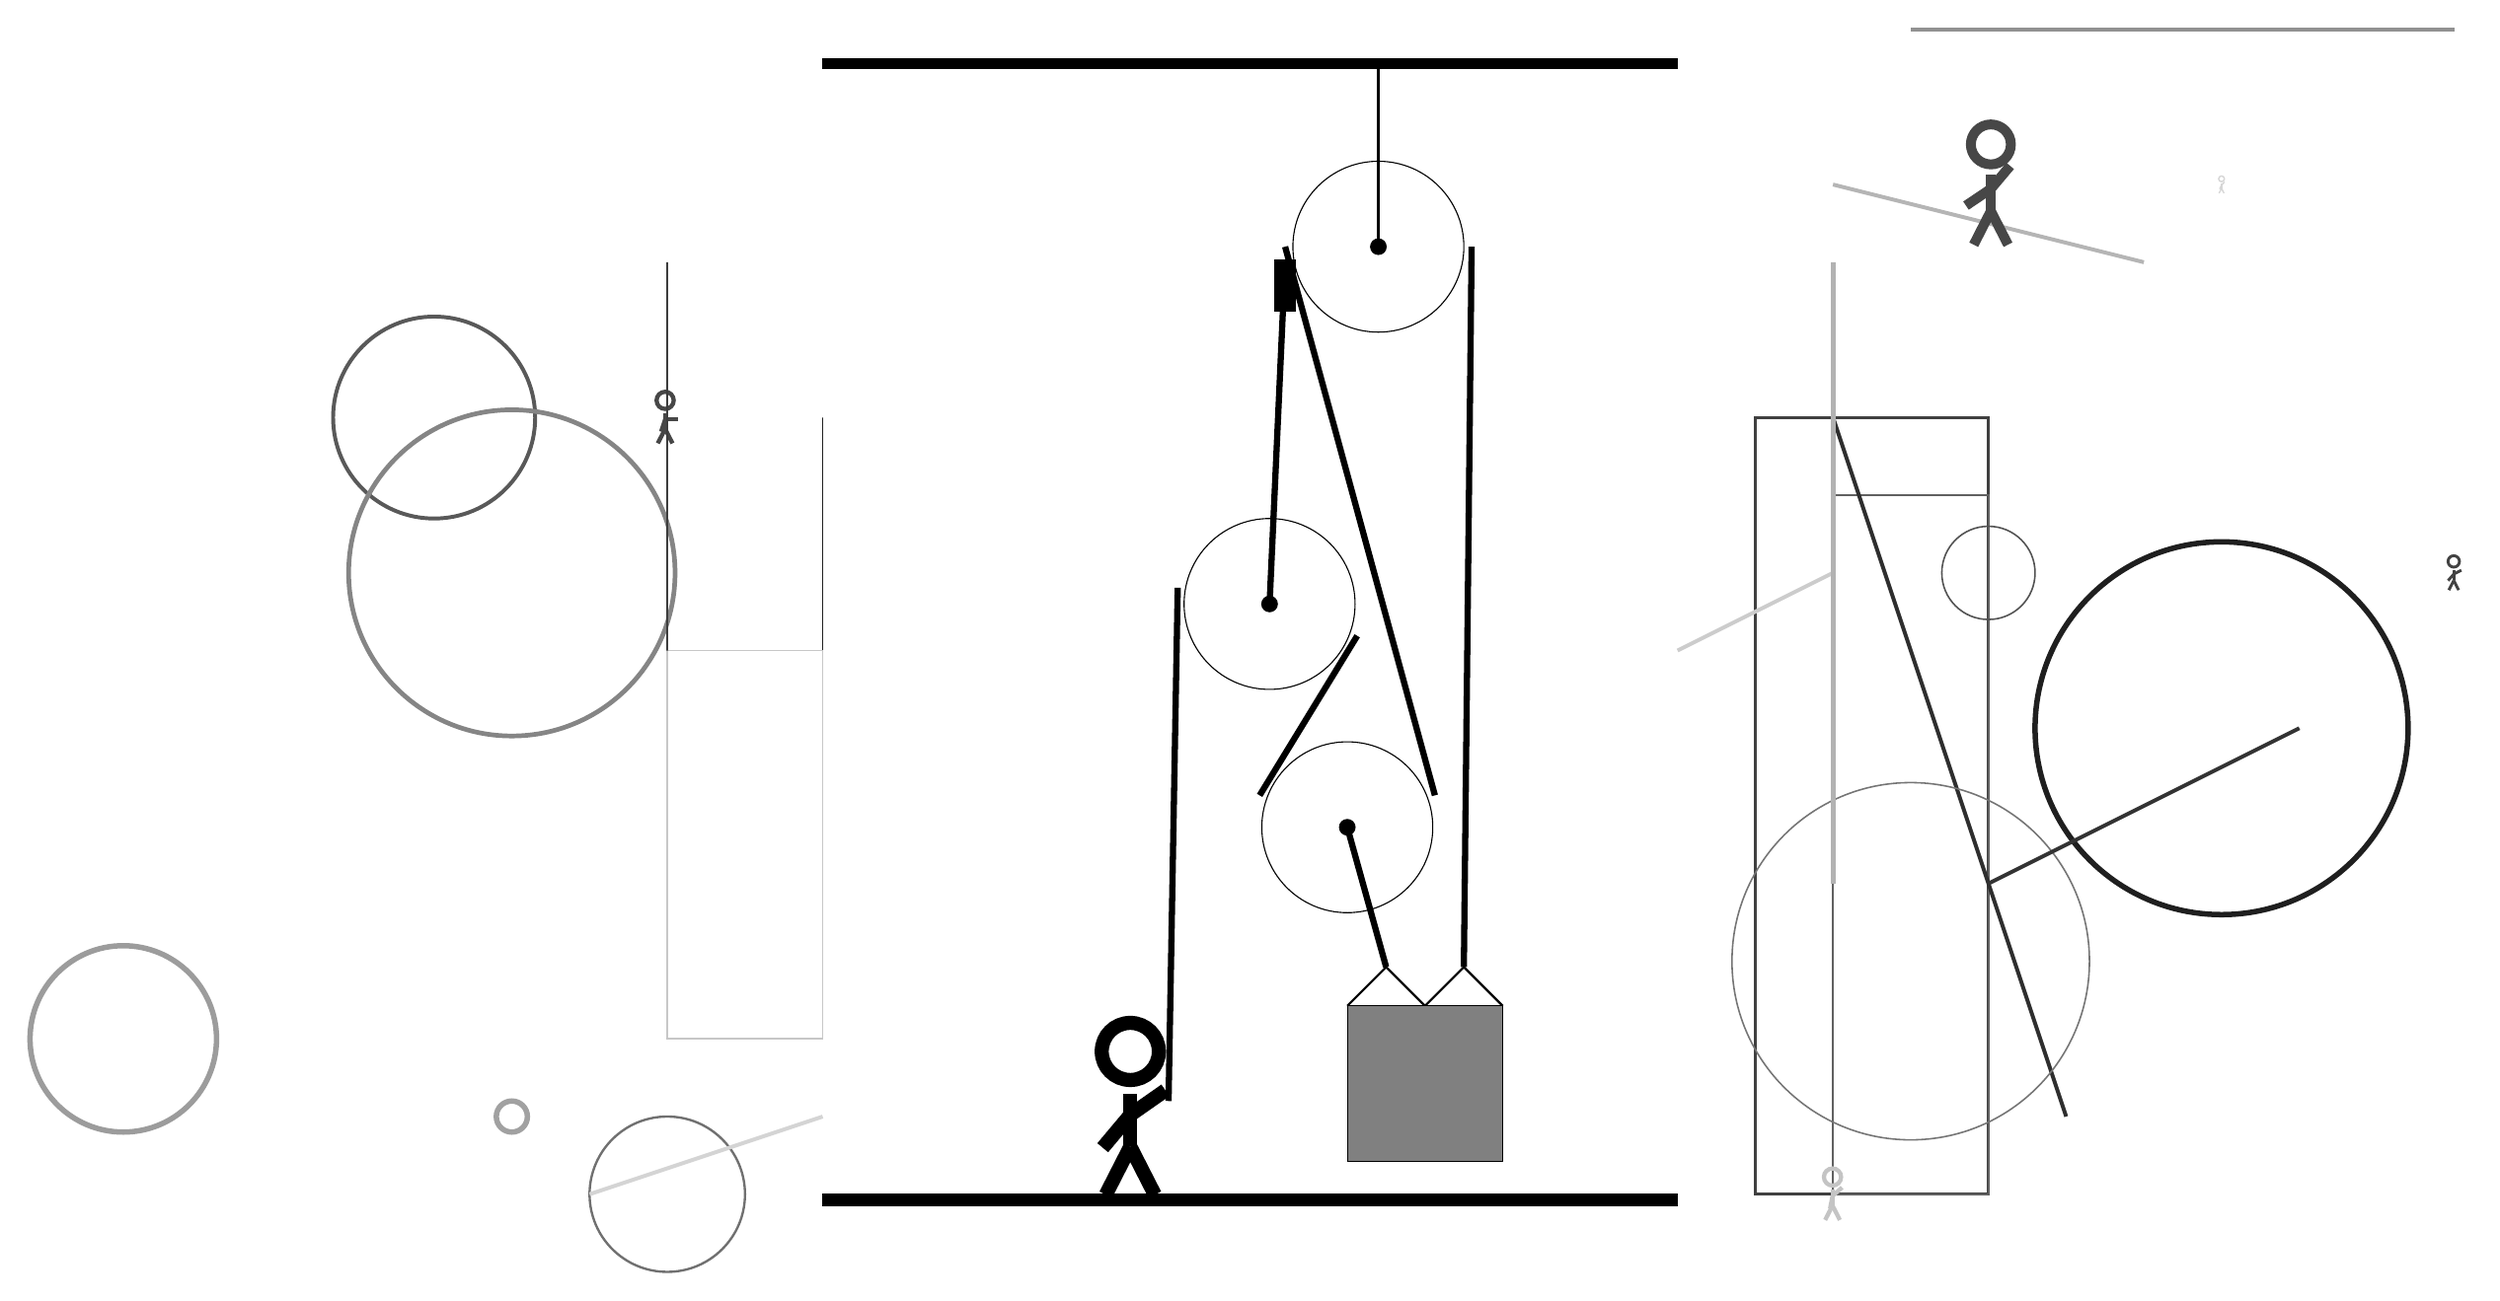
\begin{tikzpicture}
			%%%%% START %%%%%
			
			\draw[fill=black] (-6, 11.5) rectangle (5, 11.625);
			
			\draw (-0.25, 4.6) circle (1.1);
			\draw[fill=black] (-0.25, 4.6) circle (0.1);
			
			\draw (0.75, 1.725) circle (1.1);
			\draw[fill=black] (0.75, 1.725) circle (0.1);
			
			\draw (1.15, 9.2) circle (1.1);
			\draw[fill=black] (1.15, 9.2) circle (0.1);
			\draw[very thick] (1.15, 9.2) -- (1.15, 11.5);
			
			\draw[line width=0.4mm, color=black!75] (6, -3) rectangle (9, 7);
			
			\draw[line width=0.5mm, color=black!20](5, 4) -- (7, 5);
			\draw[line width=0.5mm, color=black!43](8, 12) -- (15, 12);
			\draw [line width=0.7mm, color=black!39](-15, -1) circle (1.2);
			\draw[line width=0.3mm, color=black!62] (7, 6) rectangle (9, -3);
			\draw [line width=0.3mm, color=black!56](-8, -3) circle (1.0);
			\draw[line width=0.5mm, color=black!82](7, 7) -- (10, -2);
			\draw [line width=0.7mm, color=black!88](12, 3) circle (2.4);
			\draw [line width=0.2mm, color=black!54](8, 0) circle (2.3);
			\node[line width=0.4mm, color=black!72] at (-8, 7) {\Strichmaxerl[3][72][0]};
			\draw[line width=0.2mm, color=black!87] (-6, 7) rectangle (-6, 0);
			\node[line width=0.4mm, color=black!16] at (12, 10) {\Strichmaxerl[1][63][47]};
			\draw [line width=0.2mm, color=black!68](9, 5) circle (0.6);
			\draw[line width=0.5mm, color=black!17](-6, -2) -- (-9, -3);
			\draw[line width=0.5mm, color=black!29](7, 10) -- (11, 9);
			\draw [line width=0.5mm, color=black!65](-11, 7) circle (1.3);
			
			\node[line width=0.3mm, color=black!74] at (15, 5) {\Strichmaxerl[2][49][27]};
			\node[line width=0.2mm, color=black!72] at (9, 10) {\Strichmaxerl[7][34][50]};
			\draw [line width=0.6mm, color=black!48](-10, 5) circle (2.1);
			\draw [line width=0.7mm, color=black!37](-10, -2) circle (0.2);
			\draw[line width=0.5mm, color=black!80](9, 1) -- (13, 3);
			
			\draw[line width=0.2mm, color=black!22] (-6, 4) rectangle (-8, -1);
			
			\draw[line width=0.2mm, color=black!76] (-8, 4) rectangle (-8, 9);
			\draw[line width=0.6mm, color=black!30] (7, 1) rectangle (7, 9);
			\node[line width=0.2mm, color=black!23] at (7, -3) {\Strichmaxerl[3][79][42]};
			
			
			\draw[thick]  (0.75, -0.575) -- (1.25, -0.075) -- (1.75, -0.575) -- (2.25, -0.075) -- (2.75, -0.575);
			\draw[fill=black!50] (0.75, -0.575) rectangle (2.75, -2.575);
			
			\draw[line width=0.8mm] (-0.25, 4.6) -- (-0.05, 9.0);
			\draw[line width=0.8mm, fill=black](-0.15, 8.4) rectangle (0.05, 9.0);
			\draw[line width=0.8mm] (-1.55, -1.8) -- (-1.4318, 4.8083);
			\centerarc[line width=0.8mm](-0.25, 4.6)(-20:170:1.2000000000000002);
			\draw[line width=0.8mm] (0.8776, 4.1896) -- (-0.3776, 2.1354);
			\centerarc[line width=0.8mm](0.75, 1.725)(160:380:1.2000000000000002);
			\draw[line width=0.8mm] (1.8776, 2.1354) -- (-0.05, 9.2);
			\draw[line width=0.8mm](0.75, 1.725) -- (1.25, -0.075);
			\centerarc[line width=0.8mm](1.15, 9.2)(0:180:1.2000000000000002);
			\draw[line width=0.8mm] (2.35, 9.2) -- (2.25, -0.075);
			
			\node at (-2, -1.9) {\Strichmaxerl[10][50][35]};
			
			\draw[fill=black] (-6, -3) rectangle (5, -3.15);
			
			%%%%% END %%%%%
		\end{tikzpicture}
	\end{figure}	
\end{document}